\documentclass{SGGW-thesis}

\INZYNIERSKAtrue
\WZIMtrue

\title{Zastosowanie metod uczenia maszynowego do stworzenia sztucznej inteligencji w turowych grach RPG}
\Etitle{The use of machine learning methods to create artificial intelligence in turn-based RPG games}
\author{Rafał Kuligowski}
\date{2023}
\album{205835}
\thesis{Praca dyplomowa na kierunku:}
\course{Informatyka}
\promotor{dra Marka Karwańskiego}
\pworkplace{Instytut Informatyki Technicznej\\Katedra Zastosowań Matematyki}

\renewcommand{\thefigure}{\arabic{figure}}
\renewcommand{\thetable}{\arabic{table}}
\usepackage[bottom]{footmisc}
\usepackage{hyperref}
\usepackage{subfigure}
\usepackage{float}
\usepackage{listings}
\usepackage{cite}
\raggedbottom

\begin{document}

\makeatletter
\g@addto@macro{\UrlBreaks}{%
\do\/\do\a\do\b\do\c\do\d\do\e\do\f%
\do\g\do\h\do\i\do\j\do\k\do\l\do\m%
\do\n\do\o\do\p\do\q\do\r\do\s\do\t%
\do\u\do\v\do\w\do\x\do\y\do\z%
\do\A\do\B\do\C\do\D\do\E\do\F\do\G%
\do\H\do\I\do\J\do\K\do\L\do\M\do\N%
\do\O\do\P\do\Q\do\R\do\S\do\T\do\U%
\do\V\do\W\do\X\do\Y\do\Z}
\makeatother

\maketitle
\statementpage
\abstractpage
{Zastosowanie metod uczenia maszynowego do stworzenia sztucznej inteligencji w turowych grach RPG}
{Tematem pracy było zaimplementowanie sztucznej inteligencji uczącej się za pomocą metod uczenia maszynowego w turowej grze RPG. 
Wytrenowany model ma sam podejmować decyzje o używanych akcjach w środowisku gry. Praca składa się z pięciu głównych części.
Pierwsza część omawia technologie wykorzystane w pracy oraz ich alternatywy. Druga część skupia się prezentacji gotowej aplikacji.
Trzecia część to opis techniczny wybranych elementów aplikacji. Czwarta część zawiera instrukcję użytkowania gotowej aplikacji. 
W piątej części znajduje się podsumowanie, zawierające wyniki oraz wnioski wynikające z implementacji rozwiązania.}
{uczenie maszynowe, sztuczna inteligencja, gry RPG, uczenie przez wzmacnianie, turowe systemy walki}
{The use of machine learning methods to create artificial intelligence in turn-based RPG games}
%TODO: zupdateować angielskie tłumaczenie
{The topic of the paper was the implementation of artificial intelligence, which learns through machine learning methods, in a turn-based RPG game.
The trained model is supposed to make decisions about the actions used in the game environment on its own.
The paper consists of five main parts. The first part discusses the technologies used in the work and their alternatives. The second part focuses on the presentation of the finished application.
The third part is a technical description of selected application elements. The fourth part contains user instructions for the finished application. The fifth part includes 
a summary containing the results and conclusions drawn from the implementation of the solution.}
{machine learning, artificial intelligence, RPG games, reinforcement learning, turn-based battle system}


{
  % Spis treści może być złożony z pojedynczą interlinią, np. jeśli jedna linia wychodzi na następną stronę.
  % W przeciwnym razie spis treści wstawić bez powyższego rozkazu i klamry.
  \doublespacing
  \tableofcontents
}

\startchapterfromoddpage % niezależnie od długości spisu treści pierwszy rozdział zacznie się na nieparzystej stronie

\chapter{Wstęp}
Sztuczna inteligencja w ciągu ostatnich lat objęła wiele dziedzin życia i ciągle dynamicznie się rozwija. 
Jej zastosowanie jest bardzo rozległe, a jedną z branż o dużych perspektywach rozwoju tej technologii jest przemysł rozrywkowy, 
w który wchodzą gry wideo. W grach można zastosować tę technologię do generowania zadań, poziomów czy postaci \cite{proceduralgen}, 
stworzenia systemu do wykrywania graczy używających programów oszukujących w grach wieloosobowych \cite{cheating}, oraz do stworzenia 
sztucznej inteligencji dla przeciwników gracza. Ostatnie z tych przykładowych zastosowań zostanie omówione pod względem teoretycznym i praktycznym 
zgodnie z tematem pracy.

\section{Cel i zakres pracy}
Praca ma na celu zbadanie możliwości implementacji sztucznej inteligencji dla przeciwników w grach wideo z gatunku RPG\footnote{RPG (ang. Role Playing Games)
- gry, w których gracz wciela się w rolę postaci występujących w fikcyjnym świecie. Gracze ponoszą wszelkie konsekwencje swoich akcji jako postać w świecie gry.}
z turowym systemem walki\footnote{Turowy system walki - algorytm systemu walki, który zarządza kolejnością poruszania się jego uczestników przekazując możliwość wykonania akcji według uporządkowanej kolejności określonej przez ten system. Można go porównać do topologii sieciowej token ring, gdzie żądania w danym momencie może przekazywać tylko osoba posiadająca token (w przypadku turowego systemu walki token jest nazywany turą).}. 
Wynikiem pracy będą dwie aplikacje: jedna trenująca model, a druga testująca model w postaci symulatora walki. 
Treść pracy będzie stanowić opisy technologii użytych w pracy wraz z alternatywami, opis gotowego rozwiązania, opis techniczny wybranych elementów aplikacji, instrukcję obsługi napisanej aplikacji, przykładowe wyniki powstałe w wyniku uruchomienia obu aplikacji oraz wnioski poimplementacyjne.

\chapter{Technologie}
W tym rozdziale zostaną szczegółowo omówione komponenty potrzebne do stworzenia całego tytułowego projektu. Opisane są również technologie, które nie zostały użyte w projekcie aby pokazać, że implementację można przeprowadzić na wiele różnych sposobów. Według kolejności wyboru są to: 
\begin{itemize}
  \item{Rodzaj uczenia maszynowego},
  \item{Silnik do stworzenia gry oraz pakiet do uczenia maszynowego kompatybilny z silnikiem},
  \item{Wykorzystywany algorytm do uczenia maszynowego},
  \item{System walki (w przypadku tej pracy - system oparty o tury)}.
\end{itemize}


\section{Rodzaje uczenia maszynowego}
W uczeniu maszynowym można rozróżnić trzy jego główne rodzaje (w oparciu o drugi rozdział z~\cite{MachineLearningTypes}):
\begin{itemize}
  \item{Nadzorowane (ang. Supervised) - model jest trenowany na danych wejściowych oraz odpowiednich dla nich wartości wynikowych. Na ich podstawie uczy się przewidywania wyniku dla nowych, nieznanych danych wejściowych.}
  \item{Nienadzorowane (ang. Unsupervised) - model jest trenowany na samych danych wejściowych nie dostając oczekiwanych wyników. Model sam musi odkryć sens jaki stoi za danymi wejściowymi.}
  \item{Przez wzmacnianie (ang. Reinforcement) - model trenowany za pomocą interakcji agenta w wykreowanym otoczeniu. Agent wykonując akcje w otoczeniu, dostaje nagrody lub kary, które zależą od wyników jego akcji.}
\end{itemize}
W przypadku tej pracy zostanie użyty rodzaj uczenia przez wzmacnianie, z uwagi na charakterystyczną dla niego metodę uczenia przez interakcje. 
Metoda ta pasuje do gier wideo, gdyż z założenia polegają one na interakcji gracza ze światem gry. Model będzie mógł, tak jak gracz grający w grę, uczyć się wykonywania najlepszych możliwych akcji w danym momencie poprzez ingerencję w otoczenie za pomocą akcji. Większa ilość informacji na temat 
działania uczenia przez wzmacnianie jest zawarta w~\cite{ReinforcementLearning}.

\section{Silniki graficzne oraz pakiety do uczenia}
Silnik graficzny to program odpowiedzialny za generowanie grafiki na monitorze.\footnote{Definicja pochodzi ze źródła (stan na 06.01.2024r.): \url{https://www.linfo.org/graphic_engine.html}} W przypadku tworzenia gier, silnik graficzny służy do projektowania aplikacji oraz jej kompilacji. Pakiety do uczenia maszynowego to gotowe biblioteki służące do uczenia modeli sztucznej inteligencji. 
W przypadku tego projektu, pakiet do uczenia najlepiej wybrać w oparciu o używany silnik graficzny. Poniżej znajduje się lista niektórych silników graficznych wraz z kompatybilnymi pakietami do uczenia maszynowego.
\subsection{Unity z pakietem ML-Agents}
Wśród wymienionych gotowych pakietów, ML-Agents jest najstarszym rozwiązaniem (udostępnione w 2017r.\footnote{Repozytorium powstało 8.09.2017r, pierwsza wersja pakietu pochodzi z 16.09.2017r - link do repozytorium \url{https://github.com/Unity-Technologies/ml-agents}}).
Dostępne w pakiecie są dwa algorytmy uczenia przez wzmacnianie - PPO oraz SAC\footnote{Więcej informacji o tych algorytmach w rozdziale ,,\nameref{algorithms}''}. Pakiet posiada własną dokumentację\cite{MLAgentsDocs}. 
Sam silnik Unity umożliwia tworzenie aplikacji z grafiką 2D oraz 3D, operuje na języku C\# oraz ma rozbudowaną dokumentację\cite{UnityDocs}.
\subsection{Godot z pakietem RL Agents}
Godot jest silnikiem OpenSource na licencji MIT. Według dokumentacji \cite{GodotDocs}, silnik wspiera oficjalnie dwa języki programowania: autorski język GDScript oraz C\#. Twórcy za pośrednictwem technologii GDExtension zapewnili możliwość stworzenia wsparcia dla innych języków przez każdego użytkownika tego silnika.
Dzięki temu, można na tym silniku programować również w innych językach programowania takimi jak Rust, C++ czy Swift. Pakiet RL Agents jest najbardziej rozbudowanym pakietem wśród wymienionych.
Bazuje na czterech innych pakietach\footnote{Pakiety na których bazuje RL Agents - StableBaseLines3, SampleFactory, CleanRL oraz Ray rllib (stan na 06.01.2024r.)} do uczenia przez wzmacnianie
oraz wspiera ponad 12 algorytmów uczenia. Więcej informacji o RL Agents można znaleźć w artykule naukowym poświęconym tej technologii~\cite{GodotRLAgentsArticle} oraz w dokumentacji dostępnej w repozytorium projektu~\cite{GodotRLAgentsDocs}.
\subsection{Unreal Engine z pakietem Learning Agents}
W porównaniu do innych pakietów, Learning Agents jest najmłodszy (powstał na początku 2023r.) oraz najsłabiej udokumentowany. Pakiet operuje algorytmami PPO oraz BC (ang. Behavioral Cloning)\footnote{Informacja pochodzi ze źródła (stan na 06.01.2024r.): \url{https://dev.epicgames.com/community/learning/tutorials/8OWY/unreal-engine-learning-agents-introduction}}. 
Sam silnik graficzny Unreal Engine jest narzędziem z bardzo dużym wsparciem i możliwościami. Posiada możliwość programowania w języku C++ oraz funkcję Blueprints umożliwiającą programowanie wizualne (bez pisania kodu). 
Dokumentacja zarówno silnika Unreal Engine jak i pakietu Learning Agents znajduje się w~\cite{UnrealDocs}.
\subsection{Własny silnik z wykorzystaniem różnych pakietów do uczenia maszynowego}
Rozwiązanie oferujące największą swobodę, ale też najtrudniejsze w implementacji. Do stworzenia środowiska gry potrzebna jest biblioteka graficzna pomagająca stworzyć silnik np. OpenGL
lub pakiet do stworzenia aplikacji okienkowej np. PyGame. Wybierając pakiet do uczenia maszynowego warto szukać wśród pakietów Pythona, gdyż ma on ich bardzo dużo. Dla uczenia przez wzmocnienie można zastosować pakiet PyTorch\footnote{Używany w ML-Agents oraz Learning Agents}
lub też jeden z czterech pakietów wykorzystywanych przez RL Agents.
\subsection*{Wybrany silnik i pakiet do uczenia maszynowego}
Do pracy wybrałem Unity z pakietem ML-Agents przez wzgląd na moje wcześniejsze doświadczenie z Unity i językiem C\#. Uważam jednak, że dużo bardziej rozbudowany RL Agents na silniku Godot jest lepszym wyborem do tego typu projektu, gdyż daje dużo większe pole do dostosowania uczenia dla osiągnięcia lepszych rezultatów.

\pagebreak
\section{Algorytmy do uczenia maszynowego}
\label{algorithms}
Unity ML-Agents posiada dwa algorytmy uczące PPO (ang. Proximal Policy Optimization) oraz SAC (ang. Soft Actor-Critic). Pierwszy z nich jest podstawowym algorytmem używanym w pakiecie.

PPO jest algorytmem ,,on-policy'', kiedy SAC jest algorytmem ,,off-policy''. 
Samo określenie Policy odnosi się do strategii wyboru akcji przez agenta w aktualnym stanie środowiska. 
W skład tej strategii wchodzi zarówno wybór akcji agenta jak i aktualizacja modelu zależna od nagród i kar zwracanych przez środowisko po wykonaniu akcji.

Różnica między algorytmami ,,on-policy'' i ,,off-policy'' zależy od tego czy obie funkcjonalności w Policy są od siebie odseparowane. 
Jeśli Policy wybierające akcję agenta jest inne od Policy aktualizującego model to algorytm jest ,,off-policy'', 
natomiast jeśli Policy odpowiedzialne za wybór akcji jest takie same co aktualizujące model, to algorytm jest ,,on-policy''. 
Szczegółowe informacje na temat Policy znajdują się w \cite{RLBook}.

Według \cite{MLAgentsDocs} algorytm PPO jest algorytmem ogólnego przeznaczenia i jest bardziej stabilny w porównaniu z innymi algorytmami uczenia przez wzmacnianie.
Dodatkowe informacje o algorytmie PPO znajdują się w~\cite{PPOArticle}, a o SAC w~\cite{SACArticle}. 


Do projektu wybrany został algorytm PPO z uwagi na wcześniej podaną stabilność oraz fakt, że jest on algorytmem będącym ponad 6 lat w pakiecie ML-Agents co sugeruje, że jest on lepiej rozwiniętym rozwiązaniem w pakiecie.

\section{Systemy walki w turowych grach RPG}
Systemów walki turowej w grach RPG jest bardzo dużo, lecz w większości gier są one oparte o znane już systemy. Pewne elementy są jednak stałe i można je zauważyć w każdej grze z tego gatunku.
\begin{itemize}
  \item{Rozgrywka polega na wzajemnym przekazywaniu tur postaci gracza z przeciwnikami},
  \item{Podczas tury gracz oraz przeciwnicy wykorzystują swoje tury jako zasób do wykonywania akcji},
  \item{Postacie gracza oraz przeciwnicy posiadają statystyki, które określają ich cechy. Do takich statystyk może należeć np. Obrona zmniejszająca obrażenia otrzymywane przez postać, czy też Atak zwiększający zadawane obrażenia},
  \item{Postacie gracza oraz przeciwnicy posiadają umiejętności, których mogą używać zużywając tury do wykonywania akcji w środowisku gry},
  \item{Walka kończy się gdy wszystkie postacie gracza lub wszyscy przeciwnicy zginą}.
\end{itemize}
Powyższe punkty zostały oparte o własne doświadczenia z grami tego gatunku, jak i o wybrane rozdziały z~\cite{RLLearningInTBRPG, PlayerPreferencesInRPGs}. Dalej przedstawię parę róźnych podejść do walki w systemie turowym. 
Niektóre zawierają nazwy gier lub aplikacji, z których zostały zaczerpnięte, przez brak możliwości odnalezienia źródła zawierającego ustandaryzowaną nazwę danego systemu.
\subsection{RPG Maker}
RPG Maker to program do tworzenia gier RPG nie wymagający programowania. System walki w nim użyty jest dobrą bazą do tworzenia innych, 
bardziej skomplikowanych systemów przez swoją prostotę. Na początku walki jest tworzona kolejka złożona z postaci występujących na scenie 
(zarówno wrogich jak i sojuszniczych), która jest posortowana według statystyki Szybkości. Im większa owa statystyka, tym postać jest wyżej w 
kolejce i szybciej wykona ruch. Po stworzeniu kolejki gracz wybiera ruchy wszystkich sojuszniczych postaci, a po wyborze ruchu ostatniej postaci
system przechodzi przez kolejkę, uruchamiając wybrane przez gracza oraz sztuczną inteligencję przeciwników akcje. Po wszystkim, 
system daje graczowi ponowną możliwość wyboru umiejętności. System ten był również zaimplementowany w grach z serii Etrian Oddysey oraz 
pierwszych częściach Final Fantasy.
\subsection{Darkest Dungeon}
Darkest Dungeon jest grą autorstwa Red Hook Studios. System walki w niej przedstawiony jest zmodyfikowaną wersją poprzedniego systemu, jednak wprowadza większą dynamikę. 
Gdy kolejka postaci zostanie stworzona oraz postać w drużynie gracza ma aktualnie swoją turę, gracz wybiera akcję, 
którą postać ma wykonać. Po jej wybraniu, postać wykonuje akcję i przechodzi na koniec kolejki, przekazując turę następnej postaci się w 
niej znajdującej. System ten został również użyty w grach Yakuza: Like a Dragon, Like a Dragon: Infinite Wealth czy Super Mario RPG.
\subsection{Active Time Battle}
System walki charakteryzujący się tym, że każda postać na początku zaczyna z pustym paskiem tury, ładującym się w równych interwałach. 
Gdy tura jakiejś postaci zostanie w pełni naładowana, walka zatrzymuje się, a postacie z naładowaną turą wybierają akcję, jaką mają wykonać. 
Następnie pasek tury jest dalej ładowany. Gdy ładowanie dobiegnie do końca, postać wykona wybraną wcześniej akcję i resetuje ładowanie tury 
do wartości początkowej. System ten jest znany z gier Chrono Trigger, Child of Light oraz serii Final Fantasy. Dodatkowe informacje na temat systemu walki oraz jego implementacji znajdują się w~\cite{ATB,PlayerPreferencesInRPGs}.
\subsection{Press Turn System}
Jest to nazwa systemu walki opracowanego przez firmę Atlus na potrzeby gry~\cite{SMT3}. Opiera się na zwiększeniu znaczenia tury jako zasobu poprzez rozdzielenie tur na zwykłe i naznaczone, oraz wprowadzenie oceny ruchu postaci.
Ocena opiera się na 2 powiązanych ze sobą kryteriach:
\begin{enumerate}
  \item{Rodzaj obrażeń - np. żywioły typu ogień, woda, ziemia itp.},
  \item{Relację postaci do użytego rodzaju obrażeń}.
\end{enumerate}
Pierwotna implementacja systemu zawiera 6 typów relacji do rodzaju obrażeń:
\begin{enumerate}
  \item{Neutralna},
  \item{Słabość},
  \item{Odporność},
  \item{Niewrażliwość},
  \item{Odbicie},
  \item{Absorpcja}.
\end{enumerate}
\pagebreak
System na początku rozdziela fazę gracza oraz fazę przeciwnika. Start każdej fazy rozpoczyna się od liczenia liczby tur jaką posiada poruszają się strona. Jest to zazwyczaj liczba postaci po poruszającej się stronie, wykluczając martwe jednostki (istnieją wyjątki od tej reguły np. silniejsza, samotna jednostka otrzymuje jedną dodatkową turę).
Poza liczeniem liczby tur jest tworzona kolejka postaci w której kolejności będą się one poruszać. Gdy postać aktualnie posiadająca ruch wykona akcję zaczyna się jej ocena, która zmienia ilość posiadanych przez stronę tur.
W zależności od oceny tury mogą być odejmowane lub naznaczane. Zasady oceny wyglądają następująco:
\begin{itemize}
  \item{Jeśli postać trafi w słaby punkt innej postaci lub trafi cios krytyczny, oraz posiada 1 lub więcej zwykłych tur, zwykła tura jest naznaczana.}
  \item{Jeśli postać trafi w słaby punkt innej postaci lub trafi cios krytyczny, oraz posiada same tury naznaczone, odejmowana jest naznaczona tura.}
  \item{Trafienie niebędące trafieniem krytycznym lub trafienie w inny niż Słabość typ relacji, powoduje odjęcie tur o konkretną ich liczbę priorytetyzując tury naznaczone.}
  \item{Jeśli postać postanowi przeczekać turę, system zachowuje się tak samo jak przy trafieniu krytycznym lub trafieniu w słaby punkt.}
\end{itemize}
Gdy stronie wykonującej akcje skończą się tury, następuje zmiana stron. Więcej informacji o tym systemie walki można znaleźć w pracy licencjackiej~\cite{PTS}.

\subsection*{Wybrany system walki}
Do implementacji został wybrany system Press Turn. Mimo swojego skomplikowania (co może spowodować dłuższy czas uczenia modelu) posiada on bardzo dużo ciekawych interakcji związanych z turami, które sztuczna inteligencja będzie mogła wykorzystać na swoją korzyść.

\chapter{Opis działania aplikacji}
Projekt składa się z dwóch aplikacji:
\begin{itemize}
  \item Testującej model (symulator walki),
  \item Uczącej model.
\end{itemize}
Aplikacje nie są kompilowane do plików uruchomieniowych, gdyż działają na funkcji testowania gry w Unity.
Funkcja ta jest wymagana przez pakiet ML-Agents do uczenia modelu.
Powoduje to konieczność zainstalowania silnika Unity, aby móc uruchomić obie aplikacje.
\section{Aplikacja testująca model}
Aplikacja testująca model została stworzona w postaci symulatora walki dla systemu Press Turn. Umożliwia ona dostosowanie statystyk postaci gracza jak i przeciwnika sterowanego przez wytrenowany model.
Składa się z 3 widoków:
\begin{enumerate}
  \item Menu głównego,
  \item Kreatora postaci,
  \item Symulatora walki.
\end{enumerate}

\subsection{Menu główne}
Zawiera przycisk przechodzący do kreatora postaci, przycisk umożliwiający wyjście z aplikacji oraz menu opcji w którym jest możliwość dostosowania głośności muzyki i dźwięków w symulatorze.
Ustawienia graficzne nie były potrzebne w aplikacji przez uruchamianie jej w środowisku testowym Unity, które dostosowywuje rozdzielczość do okna aplikacji.

\begin{figure}[H]
  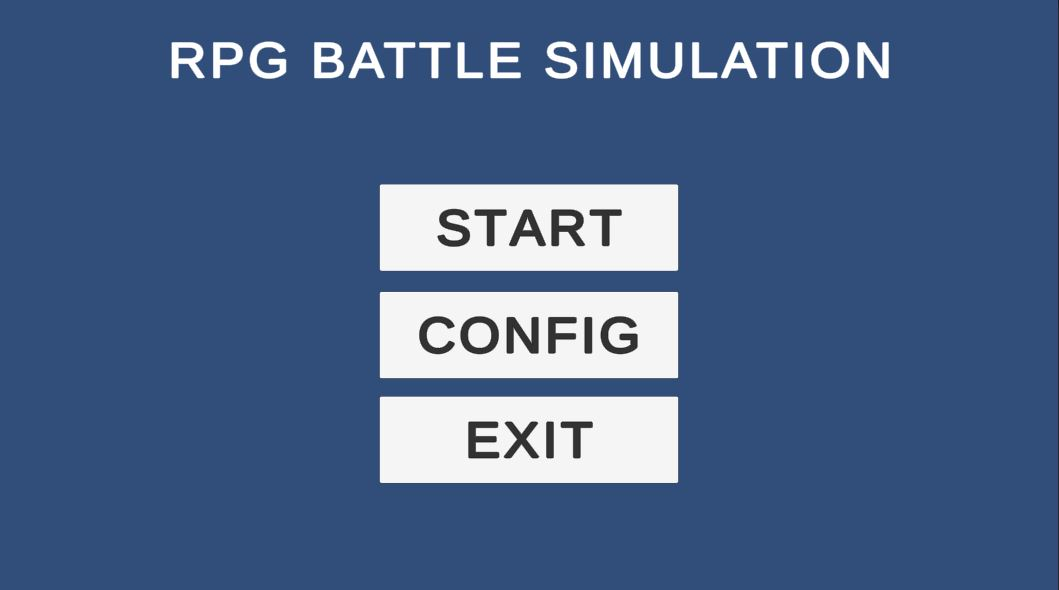
\includegraphics[width=1\textwidth]{menuscreen1.JPG}
  \caption{Widok menu głównego, \textit{Źródło: własna inicjatywa}}
\end{figure}
\begin{figure}[H]
  
\includegraphics[width=1\textwidth]{menuscreen2.JPG}
  \caption{Widok menu opcji, \textit{Źródło: własna inicjatywa}}
\end{figure}
\pagebreak
\subsection{Kreator postaci}
Kreator postaci umożliwia dostosowanie postaci według własnych potrzeb. Na początku prosi o wybranie ilości postaci po stronie gracza, następnie przechodząc do samego kreatora poszczególnych postaci gdzie można wybrać imie postaci, jej cechy, relacje z rodzajami obrażeń i umiejętności. 
Informacje o tym czym są, i za co odpowiadają te elementy kreatora znajdują się w rozdziale ,,\hyperref[systempressturn]{Walka w systemie Press Turn}''. Liczba przeciwników w każdej rozgrywce wynosi 1, aby wykluczyć zmieniającą się liczbę przeciwników, która może skomplikować proces uczenia.
\begin{figure}[H]
  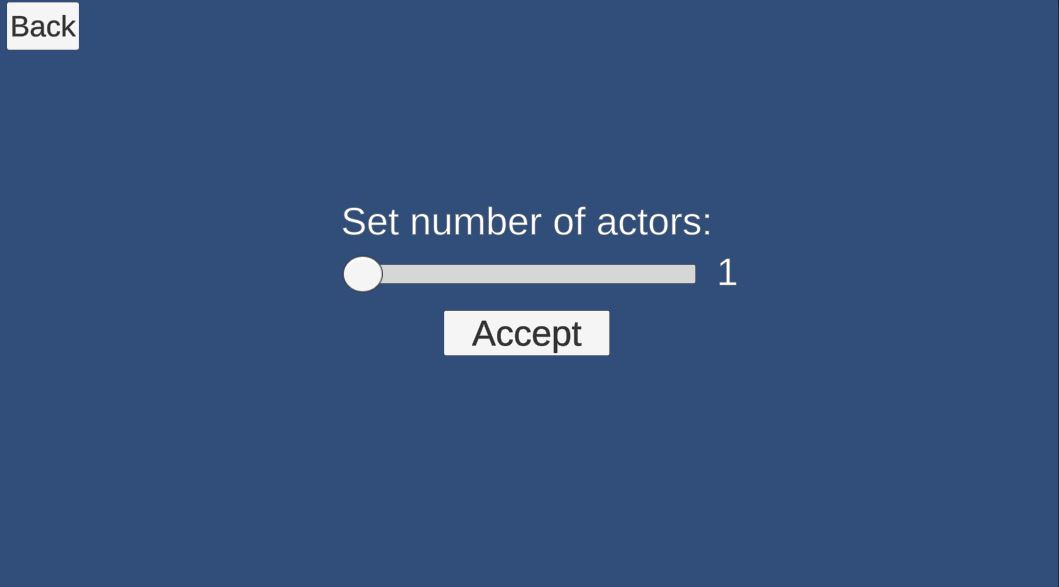
\includegraphics[width=1\textwidth]{creatorscreen1.JPG}
  \caption{Widok panelu wyboru liczby postaci, \textit{Źródło: własna inicjatywa}}
\end{figure}
\begin{figure}[H]
  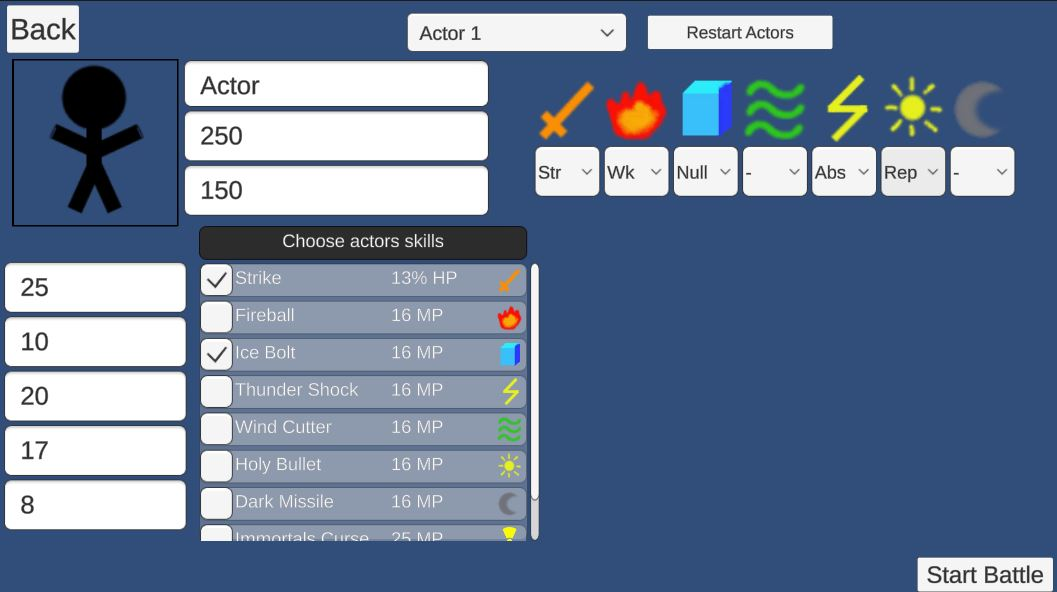
\includegraphics[width=1\textwidth]{creatorscreen2.JPG}
  \caption{Widok kreatora postaci, \textit{Źródło: własna inicjatywa}}
\end{figure}
\subsection{Symulator walki}
Symulator walki służy do testowania modelu za pomocą walki testowej gracza z przeciwnikiem sterowanym przez wytrenowany model. Walka odbywa się we wcześniej wybranym systemie Press Turn.
Widok symulatora zawiera prawie wyłącznie elementy informujące o aktualnym stanie walki. Są to:
\begin{itemize}
  \item Ilość tur zwykłych oraz naznaczonych,
  \item Wskaźniki aktualnego stanu zdrowia oraz many postaci gracza,
  \item Wskaźnik aktualnego zdrowia przeciwnika,
  \item Widok drużyny gracza, gdzie aktualnie wykonująca akcję postać posiada obramowanie,
  \item Lista umiejętności postaci gracza, która aktualnie wykonuje ruch,
  \item Dziennik zdarzeń zawierający akcje wykonane przez uczestników walki.
\end{itemize}
Przeznaczenie wymienionych wcześniej zasobów zdrowia oraz many zostało opisane w rozdziale ,,\hyperref[systempressturn]{Walka w systemie Press Turn}''.
Ułożenie elementów dla widoku symulatora zostało oparte o UI\footnote{UI (ang. User Interface, pl. Interfejs Użytkownika) - Elementy wizualne umożliwiające interakcję użytkownika z aplikacją.} sceny walki z gry \cite{SMT3}. 
\begin{figure}[H]
  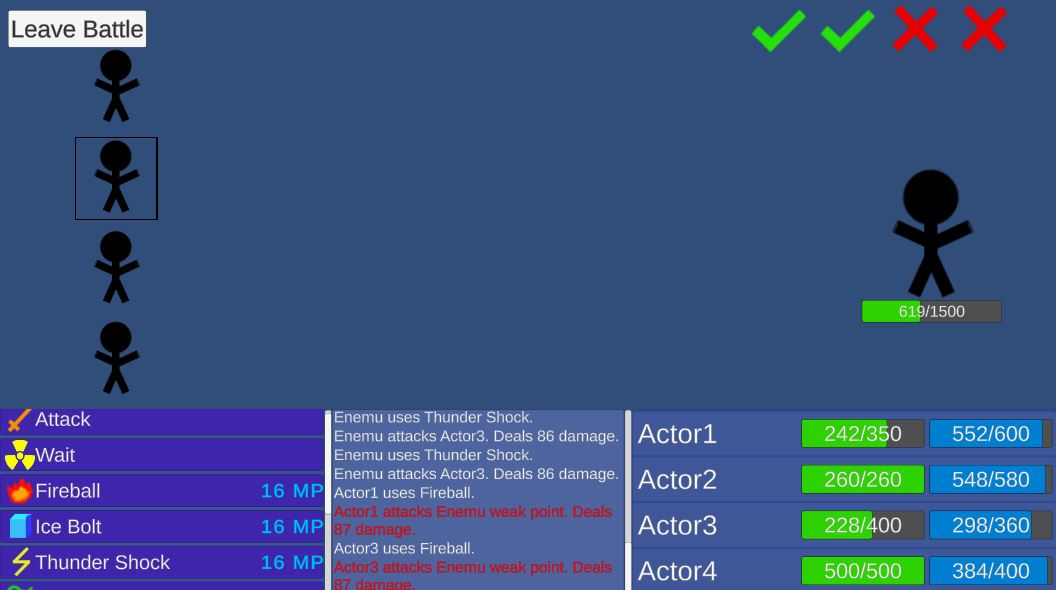
\includegraphics[width=1\textwidth]{battlescreen.JPG}
  \caption{Widok symulatora walki w projekcie, \textit{Źródło: własna inicjatywa}}
\end{figure}
\begin{figure}[H]
  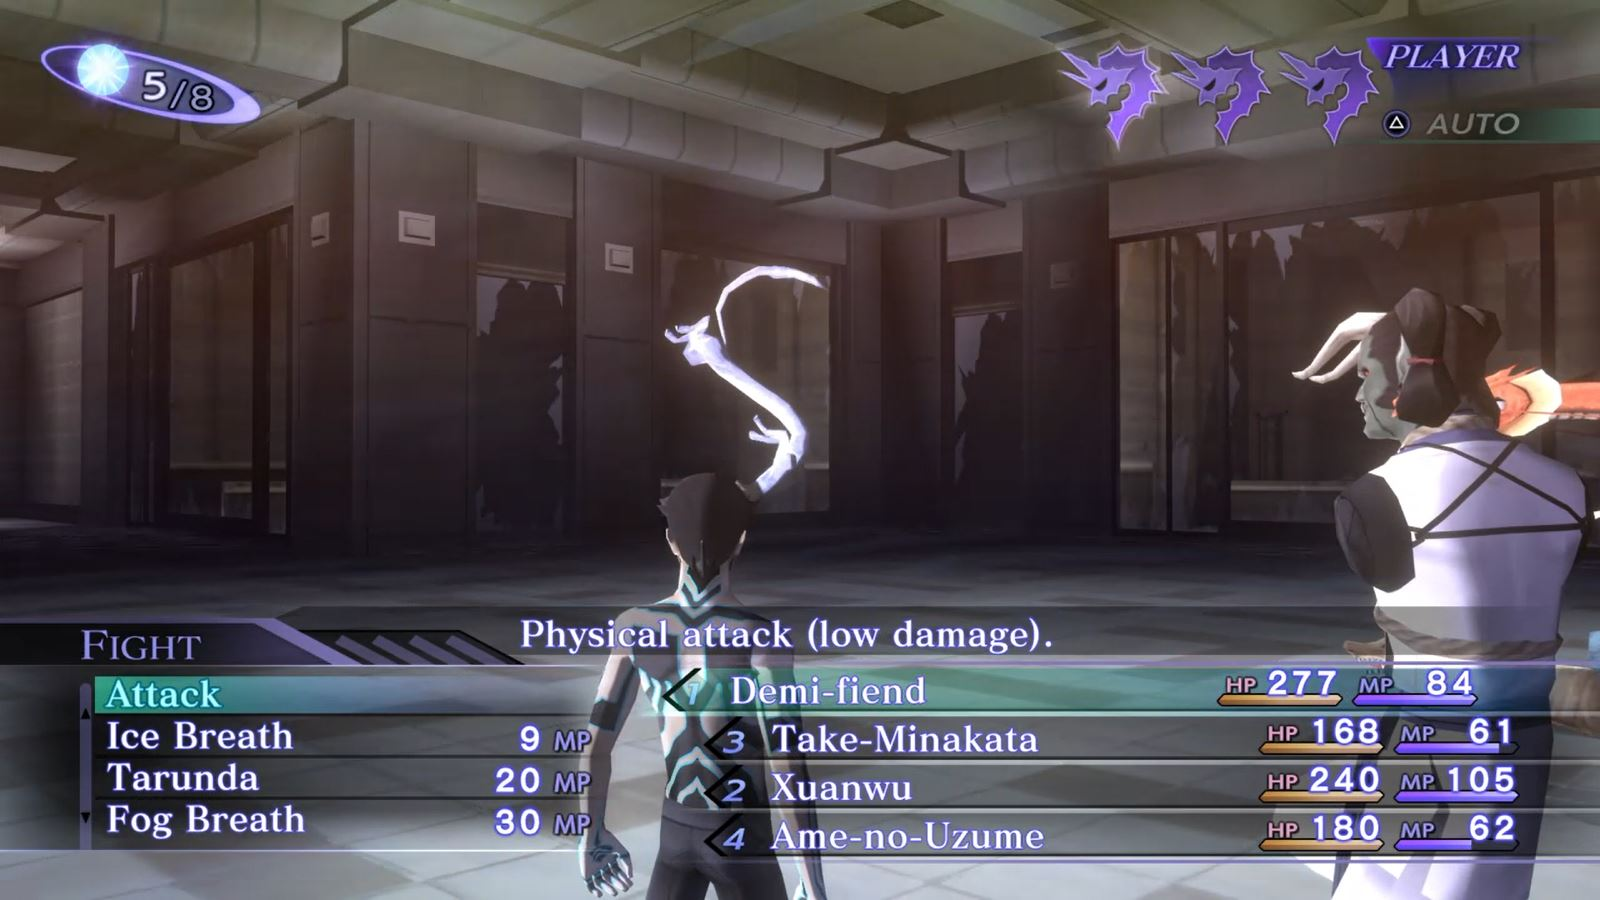
\includegraphics[width=1\textwidth]{smt3_screenshot.jpg}
  \caption{UI sceny walki z gry Shin Megami Tensei III: Nocturne, \textit{Źródło:~\cite{SMT3}}}
\end{figure}
\section{Aplikacja trenująca model}
Aplikacja trenująca model zawiera tylko jeden widok. Zawiera on element pokazujący aktualny stan środowiska uczącego oraz listę tych środowisk. 
\pagebreak

Domyślnie pokazywany jest stan pierwszego środowiska, jednak można to zmienić klikając na przycisk z nazwą innego środowiska uczącego. 
Oprócz cech postaci i informacji o turach, widocznych również w aplikacji testującej model, w widoku jest dostępny przycisk resetujący środowisko oraz informacja o ostatnio wybranej umiejętności i postaci gracza przez trenowany model.

Trening zaczyna się od wylosowania cech i umiejętności postaci przez generator liczb losowych. Proces ten wykonuje się co reset środowiska. Gdy przychodzi do tury gracza ten sam generator liczb losowych wybiera umiejętność aktualnie poruszającej się postaci.
Tury przeciwnika wykonuje trenujący się model, który jest później nagradzony lub karany za swój wybór.
Środowisko jest resetowane w przypadku wygranej bądź przegranej postaci sztucznej inteligencji, lub też jeżeli walka trwa więcej niż określona ilość tur. Proces uczenia trwa do momentu przerwania przez użytkownika aplikacji.

Ilość środowisk, zakresy losowania statystyk, nagrody, kary i liczba tur potrzebna do resetu środowiska może być dostosowana według uznania użytkownika.
\begin{figure}[H]
  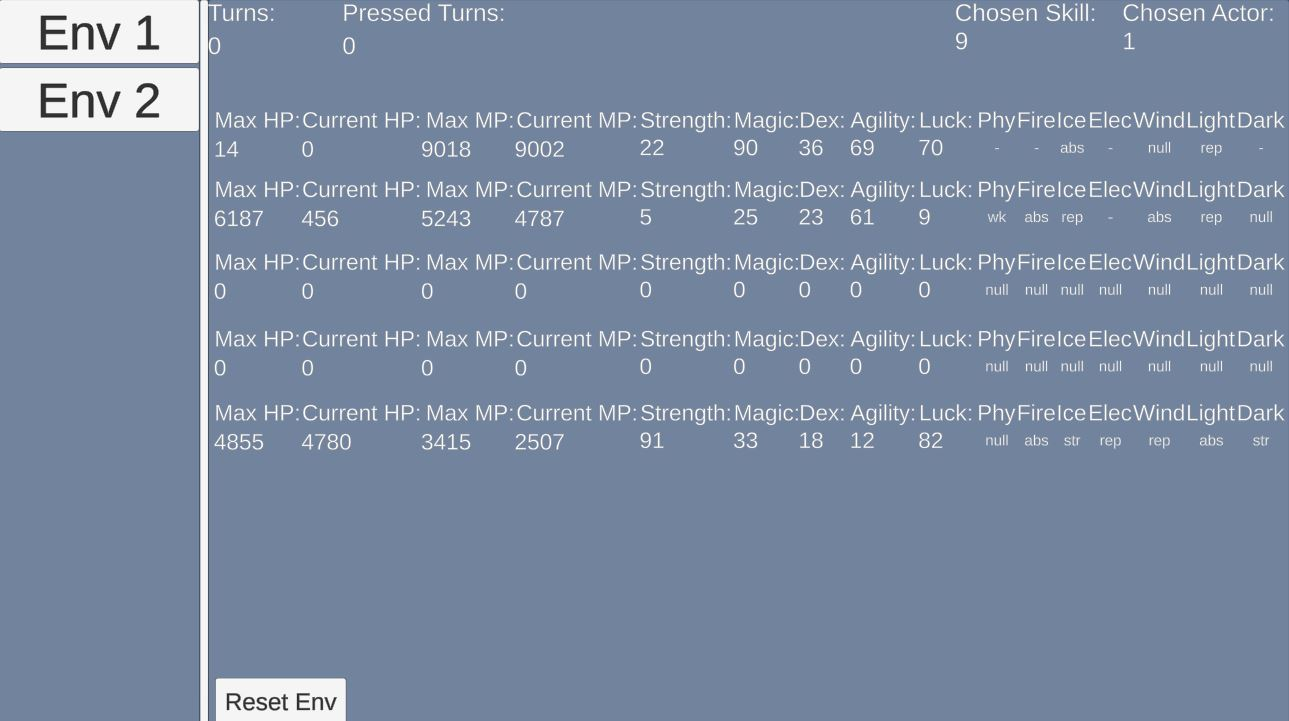
\includegraphics[width=1\textwidth]{trainingui.JPG}
  \caption{Widok UI do nadzoru trenowania modelu, \textit{Źródło: własna inicjatywa}}
\end{figure}
\pagebreak
\section{Walka w systemie Press Turn}
\label{systempressturn}
Rozdział powstał w celu uzupełnienia informacji o walce w systemie Press Turn. Są to informacje specyficzne dla implementacji dostepnej w tym projekcie. 
Rozdział opisuje:
\begin{itemize}
  \item Cechy postaci,
  \item Możliwe akcji w systemie,
  \item Rodzaje obrażeń oraz korelujące z nimi typy relacji.
\end{itemize}
\subsection{Cechy postaci}
Każda postać występująca w walce posiada te same cechy:
\begin{itemize}
  \item Punkty Zdrowia (ang. Health Points) - jest to żywotność postaci. Jeśli spadnie do 0 postać ginie. Zdrowie można tracić odnosząc obrażenia od wrogich ataków lub używając umiejętności fizycznych.
  \item Punkty Many (ang. Mana Points) - jest to zasób wykorzystywany do używania umiejętności magicznych postaci.
  \item Siła (ang. Strength) - statystyka zwiększa obrażenia od ataku podstawowego oraz umiejętności fizycznych.
  \item Magia (ang. Magic) - statystyka zwiększa obrażenia od umiejętności magicznych.
  \item Sprawność (ang. Dexterity) - statystyka zmniejsza otrzymywane obrażenia.
  \item Zwinność (ang. Agility) - statystyka definiuje miejsce w kolejce poruszania się postaci. Im większa statystyka, tym postać znajduje się wyżej w kolejce i wykona ruch przed innymi.
  \item Szczęście (ang. Luck) - statystyka w implementacji nie używana. Pierwotnie miała definiować szansę na trafienie krytyczne ataku podstawowego oraz umiejętności fizycznych lecz w finalnej wersji aplikacji mechanika nie została zaimplementowana.
\end{itemize}
Zakres wartości jakie mogą przyjąć statystyki wynosi \textlangle 1, 99\textrangle. Wyjątek stanowią zdrowie i mana które ten zakres mają szerszy - \textlangle 1, 9999\textrangle.
\pagebreak
\subsection{Akcje postaci}
Akcje postaci stanowią ich umiejętności. 
Każda umiejętność ma swój rodzaj obrażeń, koszt oraz moc podstawową. Ostatni z tych parametrów określa podstawową ilość obrażeń zadanych przez umiejętność.
Umiejętności w tej pracy trafiają zawsze tylko jeden, wybrany cel oraz mają 100\% szans na trafienie. 

Wszystkie postacie posiadają dwie podstawowe umiejętności: atak podstawowy oraz przeczekanie tury. Umiejętności te nie kosztują postaci ani zdrowia, ani many.
Reszta umiejętności to umiejętności opcjonalne, których postać nie musi posiadać. W projekcie każdy rodzaj obrażeń ma jedną umiejętność opcjonalną. 
Istnieje również umiejętność przywracająca pewną część punktów zdrowia.

\subsection{Rodzaje obrażeń i typy relacji}
Rodzajów obrażeń w implementacji jest łącznie 8. W obrębie tego projektu są one nazwywane też Elementami. Lista Elementów prezentuje się nastepująco:
\begin{enumerate}
  \item Obrażenia fizyczne,
  \item Ogień,
  \item Lód,
  \item Wiatr,
  \item Elektryczność,
  \item Światłość,
  \item Ciemność,
  \item Nadzwyczajny.
\end{enumerate}
Wszystkie Elementy, poza obrażeniami fizycznymi, powodują obrażenia magiczne. 
Elementy mają również swoje relacje. Zestawy relacji są indywidualne dla każdej postaci.
\begin{table}[H]
  \begin{center}
    \caption{Typy relacji do Elementów w projekcie wraz z ich efektami.}
  \begin{tabular}{||c c c c||} 
   \hline
   Nazwa relacji & Skrót & Wpływ na tury & Wpływ na obrażenia \\ [0.5ex] 
   \hline\hline
   Neutralny & \textit{-} & Utrata 1 tury & Brak \\ 
   \hline
   Słabość & \textit{Wk} & Naznaczenie 1 tury & +20\% \\
   \hline
   Odporność & \textit{Str} & Utrata 1 tury & -20\% \\
   \hline
   Niewrażliwość & \textit{Null} & Utrata 2 tur & Zniwelowanie obrażeń \\
   \hline
   Odbicie & \textit{Rep} & Utrata 4 tur & Odbicie wartości obrażeń \\
   \hline
   Absorpcja & \textit{Abs} & Utrata 4 tur & Wyleczenie o wartość obrażeń \\
   \hline
  \end{tabular}
  \end{center}
  \end{table}
Relacja Odbicia nie może nastąpić po raz drugi. W przypadku gdy strona przeciwna również odbija dany Element, obrażenia są niwelowane.
Dodatkowo, Element Nadzywczajny jako jedyny posiada tylko relację Neutralną.

\chapter{Opis techniczny aplikacji}
Opis techniczny zawiera szczegółowe informacje na temat wybranych elementów aplikacji. Powstał on w celu rozszerzenia informacji na temat uczenia modelu oraz implementacji systemu walki o konkretne rozwiązania programistyczne użyte w projekcie.
\section{Implementacja systemu walki}
System Press Turn opiera się o dwa nowo utworzone obiekty: BattleManager oraz BattleData. BattleManager odpowiada za logikę walki, a BattleData jest bazą postaci oraz umiejętności.
\subsection{Przygotowanie sceny walki}
Obiekt BattleData jest tworzony w kreatorze postaci przed wczytaniem się sceny symulatora walki. Bazowo zawiera on listę wszystkich umiejętności dostępnych w projekcie oraz listę stanów postaci (jedyny zaimplementowany stan to stan Śmierci). 
Uzpełniany jest dodatkowy o dwie listy:
\begin{itemize}
  \item party - przechowującą postaci sterowane przez gracza,
  \item enemies - przehcowują postać przeciwnika.
\end{itemize}
Gdy scena zostaje wczytana, inicjowany jest BattleManager, który posiada następujące właściwości:
\begin{itemize}
  \item{selectedSkill - przechowuje informacje na temat wybranej przez postać umiejętności},
  \item{isPlayerTurn - wartość prawda/fałsz mówiąca czy rusza się gracz, bazowo ustawiona na prawdę},
  \item{isBusy - wartość prawda/fałsz odpowiadająca za przejście do następnego stadium walki, bazowo ustawiona na prawdę},
  \item{gameState - enumerator mówiący jakie jest stadium walki, może przyjąć jedną z następujących wartości: START\_SIDE, START\_TURN, END\_SIDE, END\_TURN},
  \item{currentCharacter - przechowuje informacje o aktualnie poruszającej się postaci},
  \item{moveQueue - lista z indeksami postaci ułożona w kolejności poruszania się (sortowana po statystyce Agility, od największej wartości do najmniejszej)},
  \item{currentIndex - wartość pomocnicza przechowująca indeks aktualnie poruszającej się postaci},
  \item{turnQueue - lista z wartościami prawda fałsz odpowiadająca ilości tur (zwykłe tury to wartości true, naznaczone tury to wartości false)}.
\end{itemize}
Po wczytaniu wszystkich zasobów, BattleManager ustawia właściwości gameState na START\_SIDE oraz isBusy na false.
Jest to sygnał dla głównej pętli systemu walki, że może zacząć działać.

\subsection{Główna pętla systemu walki}
Główna pętla systemu walki, wbrew swojej nazwie, nie opiera się na strukturze pętli dostępnej w języku C\#. Jest to algorytm, który ma za zadanie zapętlić rozgrywkę.
W tej implementacji algorytm wykorzystuje funkcję Update wbudowaną w silnik Unity, która wykonuje się co wygenerowanie klatki przez silnik tak, aby uruchamiła się odpowiednia funkcja systemu Press Turn w zależności od stanu walki.
\begin{figure}[H]
  \centering
  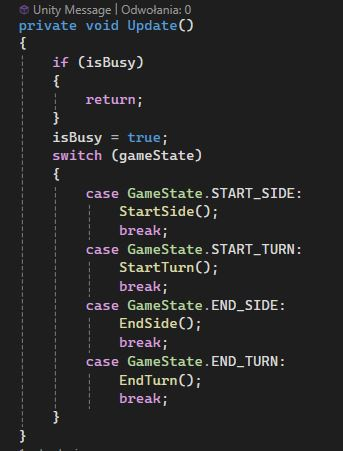
\includegraphics[height=10cm]{updatebattle.JPG}
  \caption{Funkcja Update w obiekcie BattleManager, \textit{Źródło: własna inicjatywa}}
\end{figure}
\pagebreak
Opisana pętla gry, przedstawiona w postaci listy kroków, prezentuje się nastepująco:
\begin{enumerate}
  \item{Wywołuje się StartSide(), które uzupełnia listę tur - turnQueue oraz listę indeksów postaci - moveQueue},
  \item{Następuje aktualizacja currentIndex o pierwszy indeks z moveQueue, przenosząc ten index później na koniec listy moveQueue. Potem zmienia gameState na START\_TURN},
  \item{Wywołuje się StartTurn(), które ustawia wartość currentCharacter na aktualnie poruszającą się postać},
  \item{Jeśli ruch wykonuje gracz aplikacja pokazuje dostępne umiejętności postaci i czeka na reakcję użytkownika},
  \item{Jeśli ruch wykonuje przeciwnik uruchamiana jest funkcja AIActions() która prosi o podjęcie decyzji wytrenowany model ML-Agents w wyborze celu oraz umiejętności},
  \item{Po wyborze umiejętności i celu wykonuje się funkcja UseSkill() uruchamiająca logikę systemu Press Turn},
  \item{Na koniec gameState jest zmieniany na END\_TURN},
  \item{Wywołuje się EndTurn(), które sprawdza warunki wygranej i przegranej (jeśli któryś z warunków jest prawdziwy, przejdź do 11.)},
  \item{Jeśli turnQueue jest puste, zmień stan na END\_SIDE, w przeciwnym wypadku przejdź do punktu 2.},
  \item{Wywołaj funkcję END\_SIDE, która zmienia wartość isPlayerTurn na przeciwną sobie i zmienia wartość gameState na START\_SIDE. Przejdź do punktu 1.},
  \item{Pokaż ekran końcowy i opuść pętlę gry}.
\end{enumerate}
\pagebreak
\subsection{Funkcja UseSkill}
Jest to kluczowa funkcja w tej implementacji systemu Press Turn. Pobiera ona zasoby potrzebne do użycia wybranej umiejętności, aktywuje tą umiejętność na wybranym celu oraz zmienia tury na podstawie oceny relacji do Elementu umiejętności.
W zależności od typu obrażeń, inna formuła obrażeń jest używana do ich przeliczenia. Formuły obrażeń prezentują się nastepująco:
\[PhysicalAttack = 5\cdot\sqrt{\frac{a.Strength}{b.Dexterity}\cdot m}\]\[MagicalAttack = 5\cdot\sqrt{\frac{a.Magic}{b.Dexterity}\cdot m}\]
gdzie
\begin{itemize}
  \item{a - postać atakująca},
  \item{b - postać broniąca się},
  \item{m - moc umiejętności}.
\end{itemize}

\section{Implementacja pakietu ML-Agents}
Aby zacząć uczyć model za pomocą techniki uczenia przez wzmocnienie potrzebne jest środowisko oraz uczący się w nim agent.
\subsection{Środowisko}
Środowiskiem dla agenta jest stworzony wcześniej system Press Turn z którego zostały usunięte elementy UI. Można ich utworzyć nieograniczoną ilość, a każde może być skonfigurowane w inny sposób aby zwiększyć jakość modelu wynikowego.

\pagebreak
Każde środowisko uczące zawiera następujące parametry pozwalające dostosować proces uczenia:
\begin{itemize}
  \item{maxTurns - maksymalna ilość tur po której środowisko powróci do stanu początkowego},
  \item{pointsMin - minimalna wartość wykorzystywana do losowania punktów zdrowia oraz punktów many postaci. Może przyjąć wartość z zakresu \textlangle 1, pointsMax)},
  \item{pointsMax - maksymalna wartość wykorzystywana do losowania punktów zdrowia oraz punktów many postaci. Może przyjąć wartość z zakresu (pointsMin, 9999\textrangle},
  \item{statMin - minimalna wartość wykorzystywana do losowania pozostałych cech postaci. Może przyjąć wartość z zakresu \textlangle 1, statMax)},
  \item{statMax - maksymalna wartość wykorzystywana do losowania pozostałych cech postaci. Może przyjąć wartość z zakresu (statMin, 99\textrangle},
  \item{minActors - minimalna wartość wykorzystywana do losowania ilości postaci po stronie gracza. Może przyjąć wartość z zakresu \textlangle 1, maxActors)},
  \item{maxActors - maksymalna wartość wykorzystywana do losowania ilości postaci po stronie gracza. Może przyjąć wartość z zakresu (minActors, 4\textrangle}.
\end{itemize}

\subsection{Agent}
Aby stworzyć agenta należy stworzyć nową klasę dziedziczącą po klasie z pakietu ML-Agents o nazwie Agent. Następnie należy określić jakie wartości agent będzie przewidywał. W przypadku tej pracy są to dwie wartości:
\begin{itemize}
  \item Indeks umiejętności, której agent ma użyć,
  \item Indeks postaci gracza, na której agent ma użyć umiejętności.
\end{itemize}
Aby agent mógł działać poprawnie w systemie turowym, trzeba było dodatkowo wyłączyć Automatyczne Kroki Środowiskowe w funkcji Awake()\footnote{Awake() - wbudowana funkcja silnika Unity uruchamiana tylko jeden raz przed pełnym załadowaniem klasy na scenie.} klasy agenta.
Powoduje to konieczność implementacji manulanego wykonania kroku środowiskowego\footnote{Krok środowiskowy - naznacza moment zmiany wartości w środowisku}.
Dalsza implementacja klasy agenta była oparta o artykuł \cite{MLAgentsStartegyGuide}

\pagebreak
\subsection{Interakcja środowiska z agentem}
Agent dokonuje interakcji w środowisku za pomocą zmienionej głównej pętli systemu walki. Została ona dostosowana pod trenowanie modelu. Zmodyfikowany algorytm wygląda następująco:
\begin{enumerate}
  \item{Wywołuje się funkcja OnEpisodeBegin() i całe środowisko jest na nowo losowane, następnie ustawiana jest wartość gameState na START\_SIDE},
  \item{Wywołuje się StartSide(), które uzupełnia listę tur - turnQueue oraz listę indeksów postaci - moveQueue},
  \item{Następuje aktualizacja currentIndex o pierwszy indeks z moveQueue, przenosząc ten index później na koniec listy moveQueue. Potem zmienia gameState na START\_TURN},
  \item{Wywołuje się StartTurn(), które ustawia wartość currentCharacter na aktualnie poruszającą się postać.},
  \item{Jeśli ruch wykonuje gracz aplikacja losuje umiejętność i cel dla aktualnej postaci},
  \item{Jeśli ruch wykonuje przeciwnik uruchamiana jest funkcja AIActions() która prosi o podjęcie decyzji trenowany model ML-Agents w wyborze celu oraz umiejętności. Po otrzymaniu wyniku wykonuje się funkcja EnvironmentStep()},
  \item{Po wyborze umiejętności i celu wykonuje się funkcja UseSkill() uruchamiająca logikę systemu Press Turn},
  \item{Na koniec gameState jest zmieniany na END\_TURN},
  \item{Wywołuje się EndTurn(), które sprawdza warunki wygranej, przegranej oraz limitu tur (jeśli któryś z warunków jest prawdziwy, przejdź do 12.)},
  \item{Jeśli turnQueue jest puste, zmień stan na END\_SIDE, w przeciwnym wypadku przejdź do punktu 3.},
  \item{Wywołaj funkcję END\_SIDE, która zmienia wartość isPlayerTurn na przeciwną sobie i zmienia wartość gameState na START\_SIDE. Przejdź do punktu 2.},
  \item{Wywołaj funkcje NotifyEndEpisode(), która daje nagrodę dla modelu i powoduje przejście do punktu 1.}
\end{enumerate}
\pagebreak
\subsection{Zmienne wybrane do uczenia}
Zmiennych uczących jest łączne 87. W ich skład wchodzą:
\begin{enumerate}
  \item{Ilość zwykłych tur},
  \item{Ilość naznaczonych tur},
  \item{Statystyki Aktora 1 - 17 zmiennych},
  \item{Statystyki Aktora 2 - 17 zmiennych},
  \item{Statystyki Aktora 3 - 17 zmiennych},
  \item{Statystyki Aktora 4 - 17 zmiennych},
  \item{Statystyki Przeciwnika - 17 zmiennych}.
\end{enumerate}
Wszystkie zmienne są poddane normalizacji według wzoru:
\[normValue = \frac{value-minValue}{maxValue-minValue}\]
W przypadku gdy aktor nie został stworzony w danym epizodzie, wszystkie 17 przypisanych do niego zmiennych przyjmuje wartość 0.

\chapter{Instrukcja instalacji i korzystania}
\section{Instalacja}
\subsection{Wymagane programy}
Aby aplikacja była poprawnie uruchamiana potrzebne są określone komponenty. W przypadku wersji innych od podanych nie ma gwarancji prawidłowego działania aplikacji.
Lista potrzebnych komponentów:
\begin{itemize}
  \item{Unity Hub - używany do instalacji silnika Unity},
  \item{Unity wersja 2022.2.11f1 - program Unity Hub sam zapyta o zainstalowanie tej wersji silnika podczas pierwszej próby uruchomienia projektu},
  \item{Python v3.9.13},
  \item{(opcjonalnie) Visual Studio 2022 lub Visual Studio Code - do edycji kodu źródłowego aplikacji}.
\end{itemize}

\subsection{Konfiguracja wirtualnego środowiska Pythona}
Wirtualne środowisko umożliwia instalacje pakietów bezpośrednio w folderze z projektem, dzięki czemu może on zostać zapisany na dysk przenośny i uruchomiony na każdym komputerze posiadającym wymienione wczesniej komponenty.
Poniższa instrukcja jest napisana z myślą o systemie operacyjnym Windows, gdyż na tym systemie aplikacja była tworzona i testowana.
Aby skonfigurować wirtualne środowisko, należy:
\begin{enumerate}
  \item{Uruchomić Wiersz Poleceń (cmd) w folderze bazowym projektu}.
  \item{Sprawdzić za pomocą wiersza poleceń swoją wersję Pythona za pomocą polecenia:
  \begin{lstlisting}
  python
  \end{lstlisting}
  jeśli jest poprawnie zainstalowany, zostanie otworzony program Python CLI pokazujący zainstalowaną wersję Pythona. Aby z niego wyjść należy użyć komendy:
  \begin{lstlisting}[language=Python]
  exit()
  \end{lstlisting}
  }
  \item{Utworzyć wirtualne środowisko za pomocą komendy:
  \begin{lstlisting}
  python -m venv venv
  \end{lstlisting}
  }
  \item{Aktywować wirtualne środowisko w wierszu poleceń za pomocą polecenia:
  \begin{lstlisting}
  venv\Scripts\activate
  \end{lstlisting}
  }
  \item{Zainstalować narzędzie pip do wirtualnego środowiska odpowiadające za pobieranie pakietów Pythona wpisując:
  \begin{lstlisting}
  python -m pip install --upgrade pip
  \end{lstlisting}
  }
  \item{Za pomocą narzędzia pip pobrać pakiet ML-Agents wpisując:
  \begin{lstlisting}
  pip install mlagents
  \end{lstlisting}
  }
  \item{Zainstalować pakiety wchodzące w skład biblioteki PyTorch wpisując:
  \begin{lstlisting}
  pip install torch torchvision torchaudio
  \end{lstlisting}
  }
  \item{Zmienić wersję pakietu protobuf, gdyż ta instalowana razem z ML-Agents nie działa poprawnie, za pomocą komendy:
  \begin{lstlisting}
  pip install protobuf==3.20.3
  \end{lstlisting}
  }
  \item{Pobrać pakiet ONNX odpowiadający za tworzenie plików przechowywujących modele wpisując polecenie:
  \begin{lstlisting}
  pip install onnx
  \end{lstlisting}
  }
  \item{Sprawdzić, czy ML-Agents zostało poprawnie zainstalowane za pomocą komendy:
  \begin{lstlisting}
  mlagents-learn -h
  \end{lstlisting}
  }
\end{enumerate}

\section{Korzystanie z aplikacji}
\subsection{Uruchomienie trenowania modelu}
Pierwszym etapem jaki trzeba wykonać jest wytrenowanie modelu. Aby to zrobić trzeba wykonać nastepujące kroki:
\begin{enumerate}
  \item{Uruchomić projekt poprzez Unity Hub}.
  \item{Otworzyć scenę TrainingScene znajdującą się w folderze Assets/Scenes}.
  \item{Na panelu Hierarchy należy wyszukać obiekt Environments. Służy on do przechowywania Środowisk uczących model}.
  \item{Sklonować obiekt Environment będący dzieckiem obiektu Environments tyle razy, ile ma być środowisk uczących}.
  \item{Skonfigurować Środowiska. Obiekt TrainingManager służy do konfiguracji losowych statystyk postaci w środowisku, a MLAgentsTrainer ustawia wartości nagród za akcje}.
  \item{Uruchomić wiersz poleceń w folderze z projektem następnie aktywując wirtualne środowisko}.
  \item{Uruchomić ML-Agents za pomocą komendy:
  \begin{lstlisting}
  mlagents-learn
  \end{lstlisting}
  Natomiast, jeśli już wcześniej model był uczony możemy zmusić ML-Agents do ponownego uczenia wpisując:
  \begin{lstlisting}
  mlagents-learn --force
  \end{lstlisting}}
  \item{Gdy ML-Agents wyświetli komunikat w którym czeka na Unity, należy uruchomić scenę TrainingScene w silniku Unity za pomocą funkcji testowania sceny}.
  \item{Gdy będziemy uważać, że model jest dostatecznie wytrenowany, należy wyłączyć testowanie sceny, a następnie zatrzymać uczenie w wierszu poleceń za pomocą skrótu klawiszowego CTRL+C.
  Po zatrzymaniu, ML-Agents wyświetli nazwę oraz ścieżkę do pliku z rozszerzeniem .onnx w której model został zapisany}.
\end{enumerate}
Wszystkie pliki wynikowe ML-Agents znajdują się w folderze results/ppo/. Podczas uczenia, w konsoli jest wypisywana wartość średnia oraz odchylenie standardowe nagrody jaką otrzymuje sztuczna inteligencja.
Do dokładniejszej analizy uczenia modelu może posłużyć aplikacja Tensorboard, lecz z uwagi na to, że pakiety wykorzystywane przez ML-Agents są przestarzałe i nie są 
kompatybilne z tymi obsługującymi wyżej wymienioną aplikację, nie zostało to rozwiązanie zaimplementowane.
\pagebreak
\subsection{Uruchomienie symulacji}
Po wytrenowaniu modelu, trzeba go przypisać do sztucznej inteligencji na scenie z symulacją. Aby to zrobić należy wykonać następujące kroki:
\begin{enumerate}
  \item{Skopiować plik z modelem o ścieżce podanej po zakończeniu uczenia do folderu Brains znajdującego się w katalogu [Ścieżka Projektu]/Assets/Data/}.
  \item{Otworzyć scenę BattleScene znajdującą się w folderze Scenes}.
  \item{Do obiektu MlAgentsAI należy przypisać wytrenowany model. Robi się to przeciągając z widoku zasobów projektu plik o rozszerzeniu .onnx do właściwości Model obiektu MlAgentsAI}.
  \item{Otworzyć scenę MainMenu i uruchomić symulację}.
\end{enumerate}
Po tych krokach można dostosować statystyki postaci gracza oraz przeciwnika i zasymulować walkę na danym modelu.

%\subsection{Sposób oceny modelu}
%Z uwagi na wcześniej wspomniany brak możliwości implementacji aplikacji Tensorboard, nie da się dokładnie sprawdzić jakości modelu. Można jednak sprawdzić czy model dokonuje poprawnych decyzji podczas różnych prób symulacji.
%W moim przypadku oceniałem czy model po zobaczeniu słabości na jakiś konkretny żywioł np. Ogień, posiadając też inne dostępne umiejętności będzie bardziej skłonny do atakowania tym typem obrażeń. 

\chapter{Podsumowanie}
\section{Przykładowy model wynikowy}
\subsection{Parametry uczenia}
Przykładowy model został wytrenowany na 3 środowiskach uczących o takich samych wartościach nagród za akcje. Nagrody mają następujące wartości:
\begin{itemize}
  \item Wygrana walka: 1.0,
  \item Przegrana walka: -1.0,
  \item Uderzenie w Element z relacją Neutralny: 0.2,
  \item Uderzenie w Element z relacją Słabość: 0.5,
  \item Uderzenie w Element z relacją Odporność: -0.1,
  \item Uderzenie w Element z relacją Niewrażliwość: -0.3,
  \item Uderzenie w Element z relacją Absorpcja: -0.5,
  \item Uderzenie w Element z relacją Odbicie: -0.5,
  \item Wyleczenie obrażeń: 0.3.
\end{itemize}
Środowiska zostały skonfigurowane według nastepujących parametrów:
\begin{itemize}
  \item Punkty Życia oraz Many aktorów są losowane dla środowiska:
  \begin{enumerate}
    \item z liczb o zakresie \textlangle 50, 300\textrangle,
    \item z liczb o zakresie \textlangle 300, 500\textrangle,
    \item z liczb o zakresie \textlangle 500, 700\textrangle,
  \end{enumerate}
  \item Statystyki aktorów są losowane dla środowiska:
  \begin{enumerate}
    \item z liczb o zakresie \textlangle 3, 20\textrangle,
    \item z liczb o zakresie \textlangle 25, 50\textrangle,
    \item z liczb o zakresie \textlangle 50, 75\textrangle,
  \end{enumerate}
  \item Ilość aktorów jest w każdym środowisku losowana z liczb o zakresie \textlangle 1, 4\textrangle,
  \item Maksymalna ilość tur na epizod uczenia została ustawiona na 400 dla każdego środowiska.
\end{itemize}
\subsection{Przebieg uczenia oraz jego wyniki}
Uczenie zostało przeprowadzone na domyślnych hiperparametrach. Trwało ono 300 000 kroków co przełożyło się na czas 4255 sekund oraz
wyniki w postaci średniej nagrody za akcję równej 0.506 oraz odchylenia standardowego o wartości 0.686.
\begin{figure}[H]
  \centering
  \noindent\makebox[\textwidth]{
    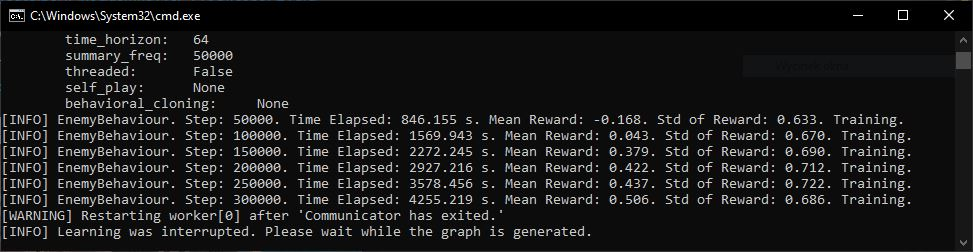
\includegraphics[width=1.1\textwidth, height=4.5cm]{results.JPG}}
  \addtocounter{figure}{6}
  \caption{Wyniki wyświetlone w aplikacji konsolowej ML-Agents, \textit{Źródło: własna inicjatywa}}
\end{figure}
\subsection{Uruchomienie i analiza zachowania modelu}
Na początku przypisałem model do sztucznej inteligencji przeciwnika oraz uruchomiłem symulator walki. Po uruchomieniu symulacji z różną konfiguracją umiejętności oraz liczbą aktorów w drużynie gracza, mogę wyodrębnić parę charakterystycznych zachowań:
\begin{itemize}
  \item Model w pierwszej kolejności skupia się na używaniu umiejętności o typie obrażeń Nadzwyczajnym. Może to być spowodowane faktem, że obrażeń z tym typem obrażeń nie da się zablokować,
  \item Jeśli model nie posiada umiejętności o typie obrażeń Nadzwyczajnym, używa naprzemiennie leczenia oraz umiejętności ofensywnych. Rzadko używa umiejętności, które mogą odebrać tury jego stronie, jednak nie wykorzystuje też zbyt często tych, które dadzą mu dodatkowe naznaczone tury.
  \item Gdy model nie ma dostępu do umiejętności leczących ani o typie obrażeń Nadzwyczajnym, zaczyna priorytetyzować słabe punkty aktorów gracza. Jeśli w danym ruchu postanowi nie zaatakować, przeczeka turę aby zyskać naznaczoną turę.
  \item Jak model nie posiada umiejętności potrafiących uderzyć w słabe punkty, najczęściej przeczekuje turę.  
\end{itemize}
\pagebreak
Wynikowy model nie jest idealny, lecz mimo to opanował on w zadowalającym stopniu zasady systemu walki. Wykorzystuje on mechanikę naznaczania tur oraz wybrał priorytetowe umiejętności zapewniające mu gwarantowane obrażenia, jak i leczenie ran.
\section{Wnioski}
Po implementacji tytułowej aplikacji oraz analizie wynikowego modelu uważam, iż jest w obecnych czasach możliwość wykorzystania technologii uczenia maszynowego w nowoczesnych grach. Wytrenowane wcześniej modele, mogłyby
zastąpić manualne tworzenie sztucznej inteligencji dla przeciwników w grach, co jednocześnie skróciłoby czas ich produkcji.
Chociaż wytrenowane wcześniej modele są realnym konceptem, który można zastosować już teraz,
to modele trenowane na bieżąco podczas rozgrywki są w tym momencie bardzo ciężkie, lub niemożliwe do zaimplementowania na technologii ML-Agents.
Jest to spowodowane wymaganymi komponentami, jakie muszą działać razem z samą grą, czyli program konsolowy uczący model w języku Python oraz środowisko testujące rozgrywkę silnika Unity.
Na stan mojej obecnej wiedzy, bez tych dwóch komponentów nie da się uruchomić uczenia modelu. Problem pojawia się również w ilości obserwacji jakich potrzebuje sieć neuronowa, aby wyciągnąć wnioski z uczenia.
Nie jest pewne, czy standardowa rozgrywka jest w stanie wyprodukować na tyle dużą ilość obserwacji dla sztucznej inteligencji, aby ta mogła nauczyć się podejmować dobre akcje w środowisku. 
%W mojej ocenie, oparcie sztucznej inteligencji w grach na przetrenowanych modelach jest w obecnych czasach możliwe. Problemem jest dodatkowe dotrenowanie lub całkowite trenowanie od podstaw modelu podczas trwania gry.
%ML-Agents wymaga uruchomionego środowiska Unity, które jest edytorem gry, aby móc trenować model co wyklucza taką możliwość. Jednak technologie uczenia maszynowego rozwijają się bardzo prężnie i jak jeszcze w roku 2020 technologie
%uczenia maszynowego były domeną naukową, bardzo mało znaną poza tym kręgiem, to aktualnie są bardzo ważną i dynamicznie rozwijaną dziedziną. Może to spowodować na tyle duży rozwój tej technologii, że uczenie sztucznej inteligencji
%podczas gry będzie możliwe.


\begin{thebibliography}{9}
  \bibitem{proceduralgen}
  Sebastian Risi, Julian Togelius
  \textit{Increasing generality in machine learning through procedural content generation},
  (2020 r.)

  \bibitem{cheating}
  José Pedro Pinto, André Pimenta, Paulo Novais
  \textit{Deep learning and multivariate time series for cheat detection in video games},
  (2021 r.)
  
  \bibitem{MachineLearningTypes}
  Shagan Sah,
  \textit{Machine Learning: A Review of Learning Types},
  (2020 r.)

  \bibitem{ReinforcementLearning}
  Vincent François-Lavet, Peter Henderson, Riashat Islam, Marc G. Bellemare, Joelle Pineau,
  \textit{An Introduction to Deep Reinforcement Learning},
  (2018 r.)

  \bibitem{MLAgentsDocs}
  \textit{Unity ML-Agents Toolkit Documentation},
  \url{https://unity-technologies.github.io/ml-agents/ML-Agents-Toolkit-Documentation/},
  (dostęp 06.01.2024r)

  \bibitem{UnityDocs}
  \textit{Unity Documentation},
  \url{https://docs.unity.com/},
  (dostęp 06.01.2024r)

  \bibitem{GodotDocs}
  \textit{Godot Documentation},
  \url{https://docs.godotengine.org/en/stable/},
  (dostęp 06.01.2024r)

  \bibitem{GodotRLAgentsArticle}
  Edward Beeching, Jilles Debangoye, Olivier Simonin, Christian Wolf,
  \textit{Godot Reinforcement Learning Agents},
  (2021 r.)

  \bibitem{GodotRLAgentsDocs}
  \textit{Godot RL Agent Repository},
  \url{https://github.com/edbeeching/godot_rl_agents/},
  (dostęp 06.01.2024r)

  \bibitem{UnrealDocs}
  \textit{Unreal Engine Documentation},
  \url{https://docs.unrealengine.com/},
  (dostęp 06.01.2024r)
  
  \bibitem{RLBook}
  Richard S. Sutton, Andrew G. Barto
  \textit{Reinforcement Learning: An Introduction, second edition},
  (2020 r.)

  \bibitem{PPOArticle}
  John Schulman, Filip Wolski, Prafulla Dhariwal, Alec Radford, Oleg Klimov, 
  \textit{Proximal Policy Optimization Algorithms},
  (2017 r.)

  \bibitem{SACArticle}
  Tuomas Haarnoja, Aurick Zhou, Pieter Abbeel, Sergey Levine, 
  \textit{Soft Actor-Critic: Off-Policy Maximum Entropy Deep Reinforcement Learning with a Stochastic Actor},
  (2018 r.)

  \bibitem{RLLearningInTBRPG}
  SangGyu Nam, Kokolo Ikeda,
  \textit{Generation of Diverse Stages in Turn-Based RolePlaying Game using Reinforcement Learning},
  (2019 r.)

  \bibitem{PlayerPreferencesInRPGs}
  Ville Mäkelä, Albrecht Schmidt,
  \textit{I Don’t Care as Long as It’s Good: Player Preferences for
  Real-Time and Turn-Based Combat Systems in Computer RPGs},
  (2020 r.)

  \bibitem{ATB}
  Agrivian Anditya, Agus Sihabuddin,
  \textit{An Optimal Input for Role-Playing Game’s
  Combat Pace using an Active Time Battle System
  Algorithm},
  (2016 r.)

  \bibitem{SMT3}
  Atlus,
  \textit{Shin Megami Tensei III: Nocturne},
  (2003 r.)

  \bibitem{PTS}
  Ryan Ganzke,
  \textit{Designing a Battle Simulator For a Popular RPG Series},
  (2023 r.)

  \bibitem{MLAgentsStartegyGuide}
  Andrew Zuo,
  \textit{Guide On Using Unity ML Agents For A Turn Based Strategy Game},
  (2021 r.),
  \url{https://andrewzuo.com/guide-on-using-unity-ml-agents-for-a-turn-based-strategy-game-9e52e6945a31/},
  (dostęp 06.01.2024r)
\end{thebibliography}

\beforelastpage

\end{document}